% ============================================
% model_template.tex
% ============================================
% Universal template for all models
% Uses generic \M... commands that get mapped to model-specific commands
% 
% IMPORTANT: Call \SetupModelTemplate{ModelWord} BEFORE inputting this file
% ============================================

\section{Performance Metrics}

\subsection{Overall Performance}

\begin{table}[h]
\centering
\caption{Overall Performance Metrics}
\begin{tabular}{lcc}
\toprule
\textbf{Metric} & \textbf{Training} & \textbf{Test} \\
\midrule
R² Score & \MRSquaredTrain & \MRSquaredTest \\
RMSE & \$\MRMSETrain & \$\MRMSETest \\
MAE & \$\MMAETrain & \$\MMAETest \\
MAPE & \MMAPETrain\% & \MMAPETest\% \\
\midrule
Sample Size & \multicolumn{2}{c}{\MTrainingSamples{} training, \MTestSamples{} test} \\
\bottomrule
\end{tabular}
\end{table}

\subsection{Accuracy Bands}

\begin{table}[h]
\centering
\caption{Prediction Accuracy Within Error Thresholds}
\begin{tabular}{lc}
\toprule
\textbf{Error Threshold} & \textbf{\% Within Threshold} \\
\midrule
Within \$1,000 & \MWithinOneK\% \\
Within \$2,000 & \MWithinTwoK\% \\
Within \$5,000 & \MWithinFiveK\% \\
Within \$10,000 & \MWithinTenK\% \\
Within \$20,000 & \MWithinTwentyK\% \\
\bottomrule
\end{tabular}
\end{table}

\subsection{Cross-Validation Results}

\begin{table}[h]
\centering
\caption{10-Fold Cross-Validation Performance}
\begin{tabular}{lc}
\toprule
\textbf{Metric} & \textbf{Value} \\
\midrule
Mean R² & \MCVMean \\
Standard Deviation & \MCVStd \\
95\% Confidence Interval & [\fpeval{\MCVMean - 1.96*\MCVStd}, \fpeval{\MCVMean + 1.96*\MCVStd}] \\
\bottomrule
\end{tabular}
\end{table}

\section{Subgroup Analysis}

\subsection{Performance by Living Setting}

\begin{table}[h]
\centering
\caption{Model Performance by Living Setting}
\begin{tabular}{lcccc}
\toprule
\textbf{Living Setting} & \textbf{N} & \textbf{R²} & \textbf{RMSE} & \textbf{Bias} \\
\midrule
Family Home (FH) & \MSubgroupLivingFHN & \MSubgroupLivingFHRSquared & \$\MSubgroupLivingFHRMSE & \$\MSubgroupLivingFHBias \\
Independent/Supported Living (ILSL) & \MSubgroupLivingILSLN & \MSubgroupLivingILSLRSquared & \$\MSubgroupLivingILSLRMSE & \$\MSubgroupLivingILSLBias \\
Residential Habilitation (RH1--4) & \MSubgroupLivingRHOneFourN & \MSubgroupLivingRHOneFourRSquared & \$\MSubgroupLivingRHOneFourRMSE & \$\MSubgroupLivingRHOneFourBias \\
\bottomrule
\end{tabular}
\end{table}

\subsection{Performance by Age Group}

\begin{table}[h]
\centering
\caption{Model Performance by Age Group}
\begin{tabular}{lcccc}
\toprule
\textbf{Age Group} & \textbf{N} & \textbf{R²} & \textbf{RMSE} & \textbf{Bias} \\
\midrule
Ages 3--20 & \MSubgroupAgeAgeUnderTwentyOneN & \MSubgroupAgeAgeUnderTwentyOneRSquared & \$\MSubgroupAgeAgeUnderTwentyOneRMSE & \$\MSubgroupAgeAgeUnderTwentyOneBias \\
Ages 21--30 & \MSubgroupAgeAgeTwentyOneToThirtyN & \MSubgroupAgeAgeTwentyOneToThirtyRSquared & \$\MSubgroupAgeAgeTwentyOneToThirtyRMSE & \$\MSubgroupAgeAgeTwentyOneToThirtyBias \\
Ages 31+ & \MSubgroupAgeAgeThirtyOnePlusN & \MSubgroupAgeAgeThirtyOnePlusRSquared & \$\MSubgroupAgeAgeThirtyOnePlusRMSE & \$\MSubgroupAgeAgeThirtyOnePlusBias \\
\bottomrule
\end{tabular}
\end{table}

\subsection{Performance by Cost Quartile}

\begin{table}[h]
\centering
\caption{Model Performance by Cost Quartile}
\begin{tabular}{lcccc}
\toprule
\textbf{Cost Quartile} & \textbf{N} & \textbf{R²} & \textbf{RMSE} & \textbf{Bias} \\
\midrule
Q1 (Low Cost) & \MSubgroupCostQOneLowN & \MSubgroupCostQOneLowRSquared & \$\MSubgroupCostQOneLowRMSE & \$\MSubgroupCostQOneLowBias \\
Q2 & \MSubgroupCostQTwoN & \MSubgroupCostQTwoRSquared & \$\MSubgroupCostQTwoRMSE & \$\MSubgroupCostQTwoBias \\
Q3 & \MSubgroupCostQThreeN & \MSubgroupCostQThreeRSquared & \$\MSubgroupCostQThreeRMSE & \$\MSubgroupCostQThreeBias \\
Q4 (High Cost) & \MSubgroupCostQFourHighN & \MSubgroupCostQFourHighRSquared & \$\MSubgroupCostQFourHighRMSE & \$\MSubgroupCostQFourHighBias \\
\bottomrule
\end{tabular}
\end{table}

\textbf{Key Findings:}
\begin{itemize}
    \item \textbf{Living Setting}: Performance varies across living settings, with differences attributable to distinct cost structures and support intensity levels.
    \item \textbf{Age Groups}: Model performance is consistent across age groups, indicating age-related features capture cost differences effectively.
    \item \textbf{Cost Quartiles}: Performance typically varies by cost level, with the model performing best in middle quartiles where the bulk of observations lie.
\end{itemize}

\section{Variance and Stability Metrics}

\begin{table}[h]
\centering
\caption{Model Variance and Stability Metrics}
\begin{tabular}{lc}
\toprule
\textbf{Metric} & \textbf{Value} \\
\midrule
Coefficient of Variation (Actual) & \MCVActual \\
Coefficient of Variation (Predicted) & \MCVPredicted \\
95\% Prediction Interval & ±\$\MPredictionInterval \\
Budget-Actual Correlation & \MBudgetActualCorr \\
\bottomrule
\end{tabular}
\end{table}

\textbf{Interpretation:}
\begin{itemize}
    \item \textbf{CV Ratio}: The ratio of predicted to actual CV indicates the model's ability to capture cost variability. Values close to 1.0 suggest the model accurately reflects population heterogeneity.
    \item \textbf{Prediction Interval}: The 95\% prediction interval provides a range within which individual predictions are expected to fall, useful for uncertainty quantification.
    \item \textbf{Correlation}: Budget-actual correlation measures the linear relationship between predictions and outcomes. High values ($>$ 0.80) indicate strong predictive validity.
\end{itemize}

\section{Population Impact Scenarios}

\begin{table}[h]
\centering
\caption{Population Served Analysis --- \$1.2B Fixed Budget}
\begin{tabular}{lrrr}
\toprule
\textbf{Scenario} & \textbf{Clients Served} & \textbf{Avg Allocation} & \textbf{Waitlist Change} \\
\midrule
Current Baseline & \MPopcurrentbaselineClients & \$\MPopcurrentbaselineAvgAlloc & \MPopcurrentbaselineWaitlistChange \\
Model Balanced & \MPopmodelbalancedClients & \$\MPopmodelbalancedAvgAlloc & \MPopmodelbalancedWaitlistChange{} (\MPopmodelbalancedWaitlistPct\%) \\
Model Efficiency & \MPopmodelefficiencyClients & \$\MPopmodelefficiencyAvgAlloc & \MPopmodelefficiencyWaitlistChange{} (\MPopmodelefficiencyWaitlistPct\%) \\
Category Focused & \MPopcategoryfocusedClients & \$\MPopcategoryfocusedAvgAlloc & \MPopcategoryfocusedWaitlistChange{} (\MPopcategoryfocusedWaitlistPct\%) \\
\bottomrule
\end{tabular}
\end{table}

\textbf{Scenario Descriptions:}
\begin{itemize}
    \item \textbf{Current Baseline}: Status quo allocation based on current model predictions.
    \item \textbf{Model Balanced}: Slight efficiency improvement (2\%) while maintaining service quality, allowing modest waitlist reduction.
    \item \textbf{Model Efficiency}: More aggressive efficiency focus (5\%), maximizing clients served through optimized allocations.
    \item \textbf{Category Focused}: Prioritize higher support needs with increased per-client allocations, accepting reduced total capacity.
\end{itemize}

\section{Model Diagnostics}

\begin{figure}[h]
    \centering
    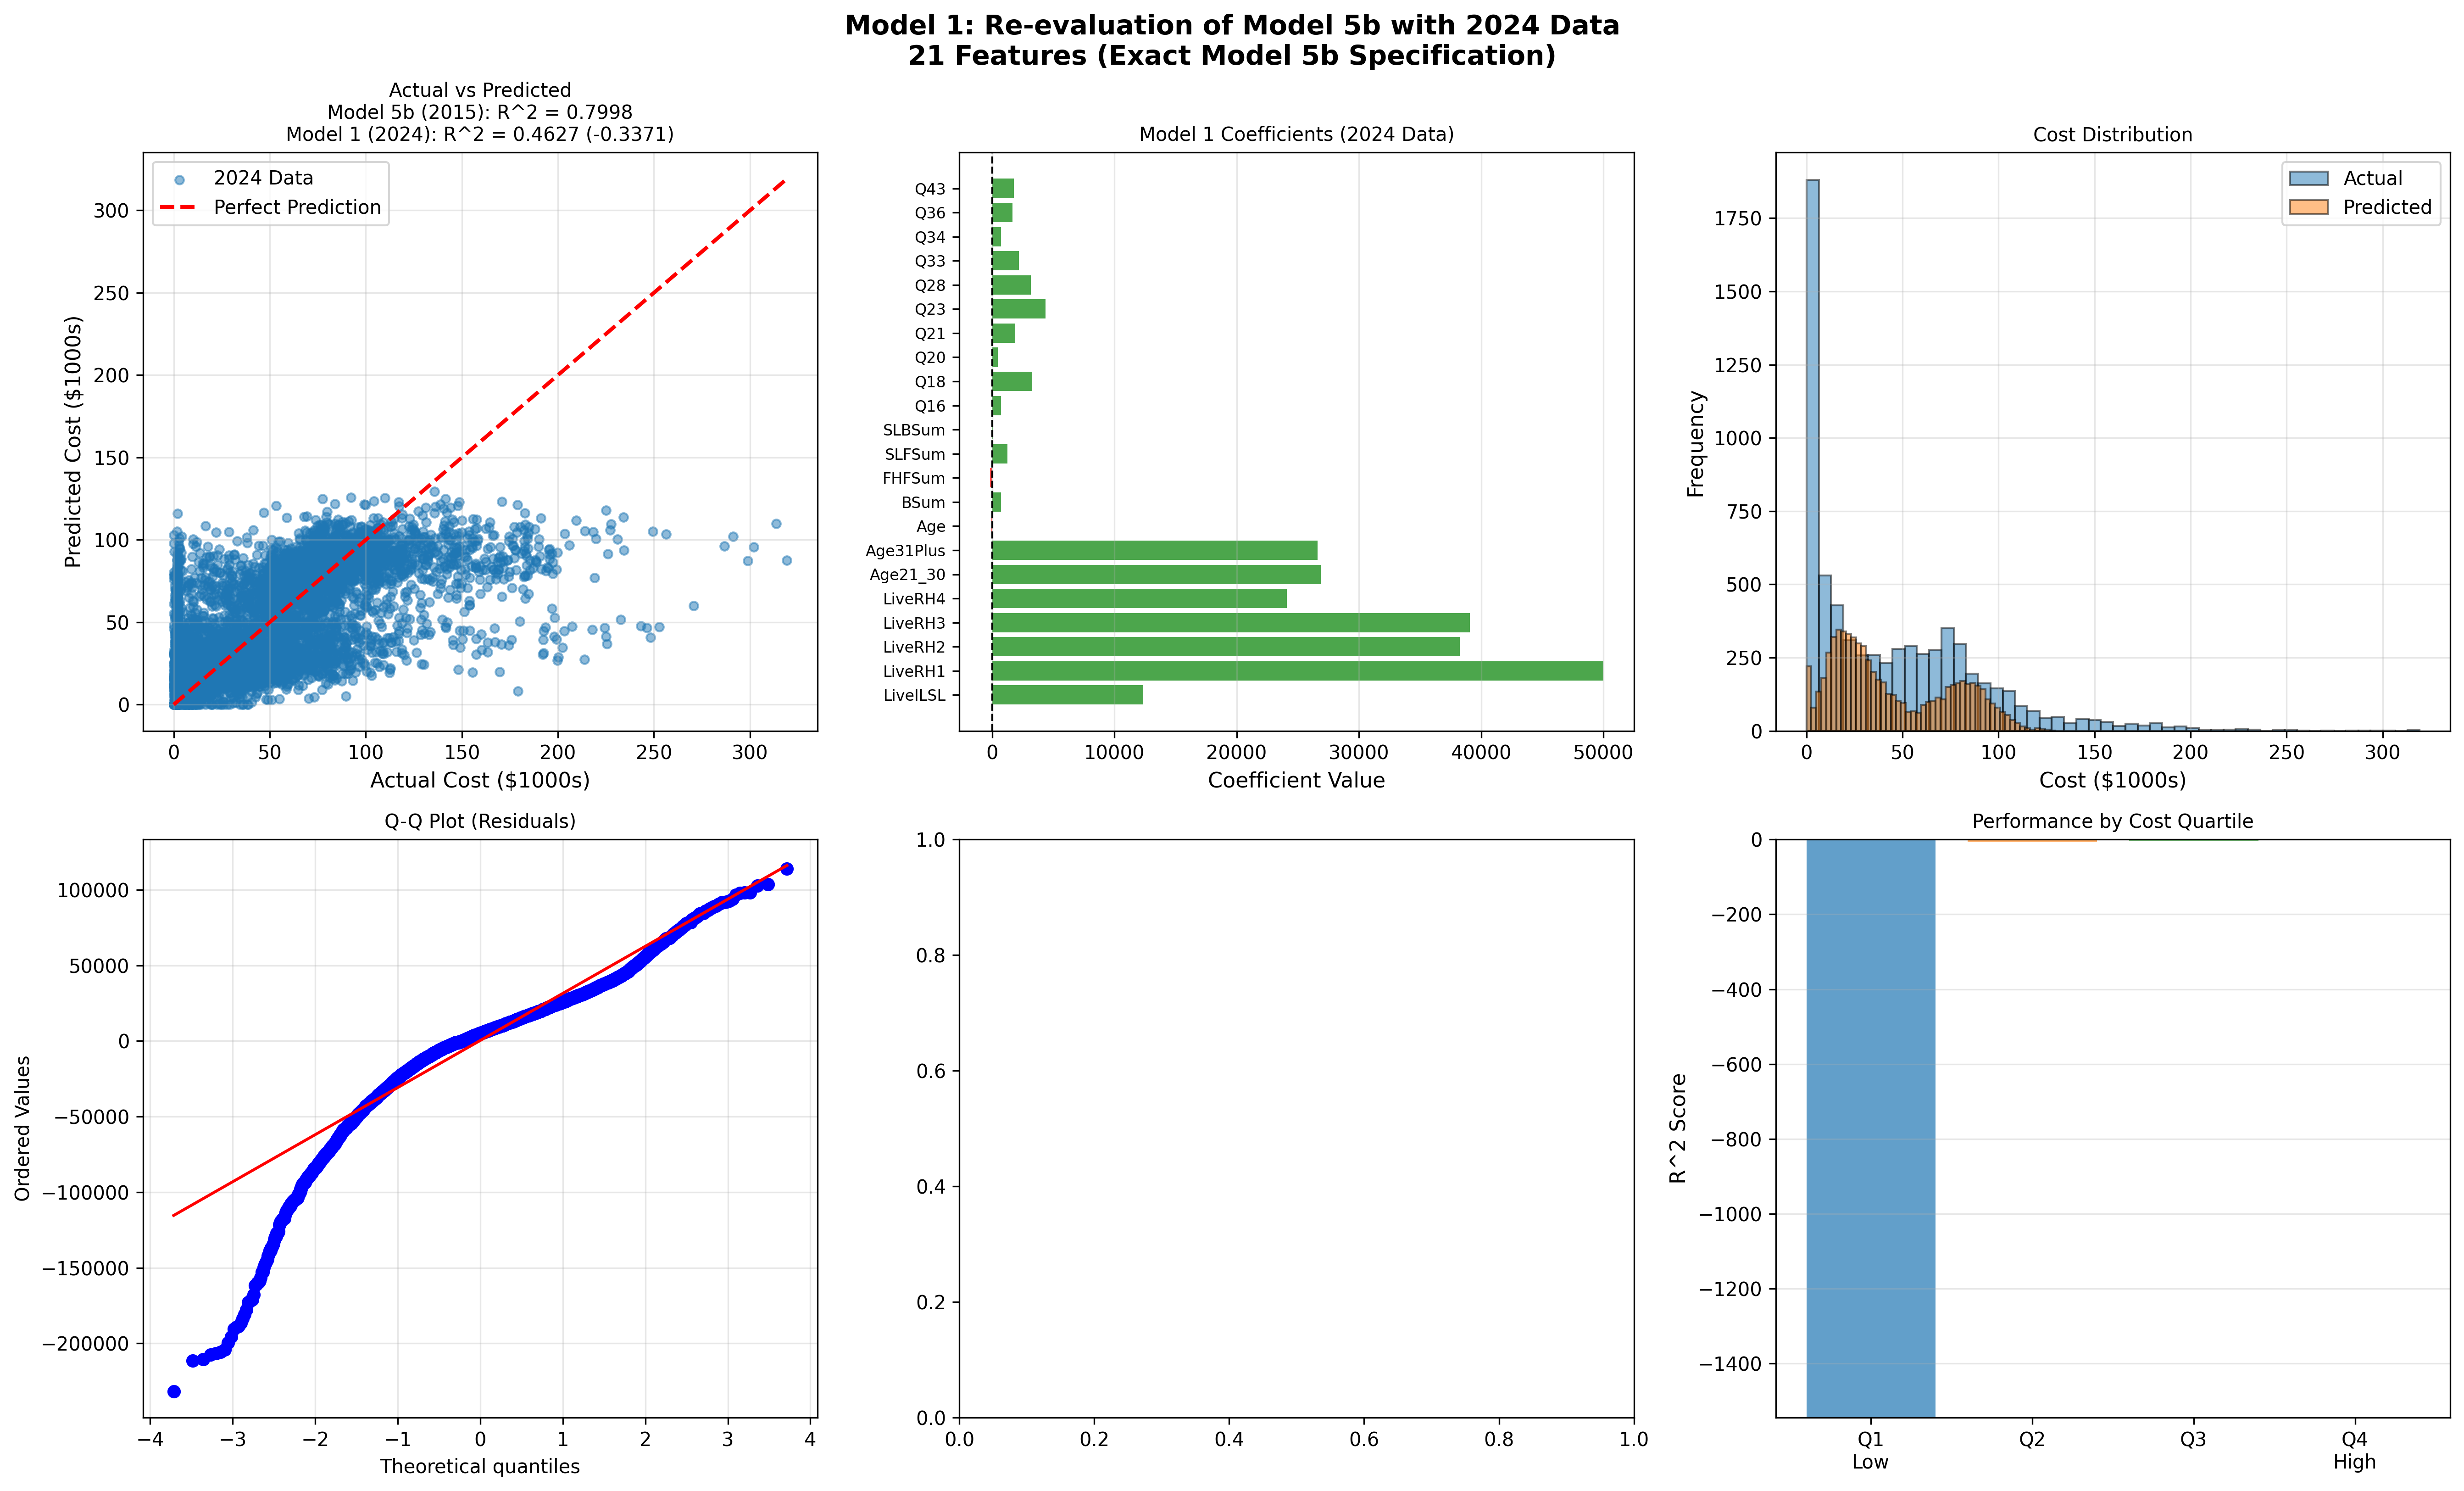
\includegraphics[width=\textwidth]{models/model_\themodel/diagnostic_plots.png}
    \caption{Model Diagnostic Plots --- Shows actual vs.\ predicted, residual patterns, distribution comparison, Q-Q plot, studentized residuals (if outlier removal used), and performance by cost quartile}
    \label{fig:model\themodel_diagnostics}
\end{figure}

\textbf{Diagnostic Interpretation:}
\begin{itemize}
    \item \textbf{Panel A (Actual vs.\ Predicted)}: Points should cluster along the 45° line. Systematic deviations indicate bias in certain cost ranges.
    \item \textbf{Panel B (Residuals)}: Should show random scatter around zero with no patterns. Funnel shapes indicate heteroscedasticity.
    \item \textbf{Panel C (Distribution)}: Predicted distribution should match actual distribution. Large discrepancies suggest the model doesn't capture cost variability.
    \item \textbf{Panel D (Q-Q Plot)}: Tests normality of residuals. Points should follow the diagonal line. Deviations at tails indicate non-normality.
    \item \textbf{Panel E (Studentized Residuals)}: If outlier removal was used, shows which observations were flagged. Should see most points within threshold bounds.
    \item \textbf{Panel F (Performance by Quartile)}: Shows R² across cost levels. Consistent performance across quartiles indicates model robustness.
\end{itemize}

% ============================================
% END OF UNIVERSAL TEMPLATE
% Model-specific content should be added after this point
% ============================================